\begin{frame}{CL ``Platform''}
  \begin{columns}
    \column{0.25\textwidth}
      \begin{tikzpicture}[x=1cm,y=2cm]
        \foreach \i in {1,...,10}
        {
          \pgfmathrand
          \let\myx=\pgfmathresult
          \pgfmathrand
          \let\myy=\pgfmathresult
          \node at (\myx, \myy) {
            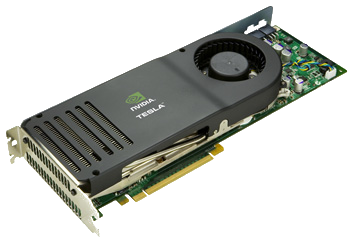
\includegraphics[width=0.6\textwidth]{c870.png}
          } ;
        }
      \end{tikzpicture}
    \column{0.75\textwidth}
    \begin{itemize}
      \item ``Platform'': a collection of devices, all from 
        the same \emph{vendor}.

      \item All devices in a platform use same CL driver/implementation.
      \item Multiple platforms can be used from one
        program $\rightarrow$ \emph{ICD}.

        \medskip
        \texttt{libOpenCL.so}: ICD loader

        \medskip
        \texttt{/etc/OpenCL/vendors/\textit{somename}.icd}:
          Plain text file with name of \texttt{.so} containing 
          CL implementation.

    \end{itemize}
  \end{columns}
\end{frame}
